% A TikZ cubic, not an addplot interpolation: the controls reach y=3.9,
% but the symmetric curve reaches only y=3.3 at x=3. Its chord is y=1.5.
% The independent naming and filling use the PGFPlots fillbetween library.
\documentclass[border=2pt]{standalone}
\usepackage{pgfplots}
\usepgfplotslibrary{fillbetween}
\pgfplotsset{compat=1.18}
\begin{document}
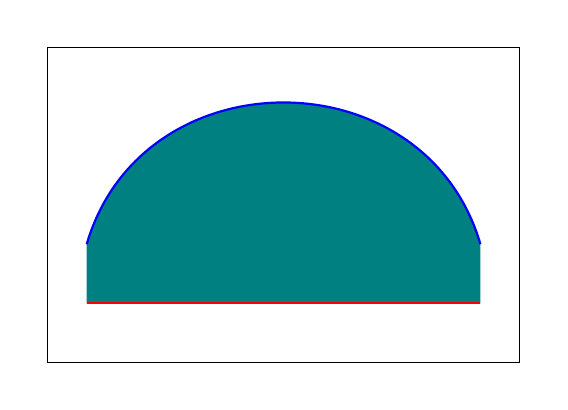
\begin{tikzpicture}
  \begin{axis}[at={(0,0)},anchor=south west,width=6cm,height=4cm,scale only axis,
    xmin=0,xmax=6,ymin=0,ymax=4,enlargelimits=false,axis lines=box,ticks=none]
    \draw[blue,thick,name path=upper] (axis cs:0.5,1.5)
      .. controls (axis cs:1.2,3.9) and (axis cs:4.8,3.9) .. (axis cs:5.5,1.5);
    \addplot[red,thick,mark=none,name path=lower] coordinates {(0.5,0.75) (5.5,0.75)};
    \addplot[draw=none,fill=teal] fill between[of=upper and lower];
  \end{axis}
  \path[use as bounding box] (-0.25,-0.25) rectangle (6.25,4.25);
\end{tikzpicture}
\end{document}
